
\documentclass[12pt, screen]{report}
%\usepackage{graphicx,color}
%\usepackage{amsmath, amssymb, amsthm}
\usepackage[margin=0pt, papersize={147mm,78mm}]{geometry}
\pagestyle{empty}

\usepackage{tikz}
\usetikzlibrary{trees,decorations.pathmorphing}
\begin{document}

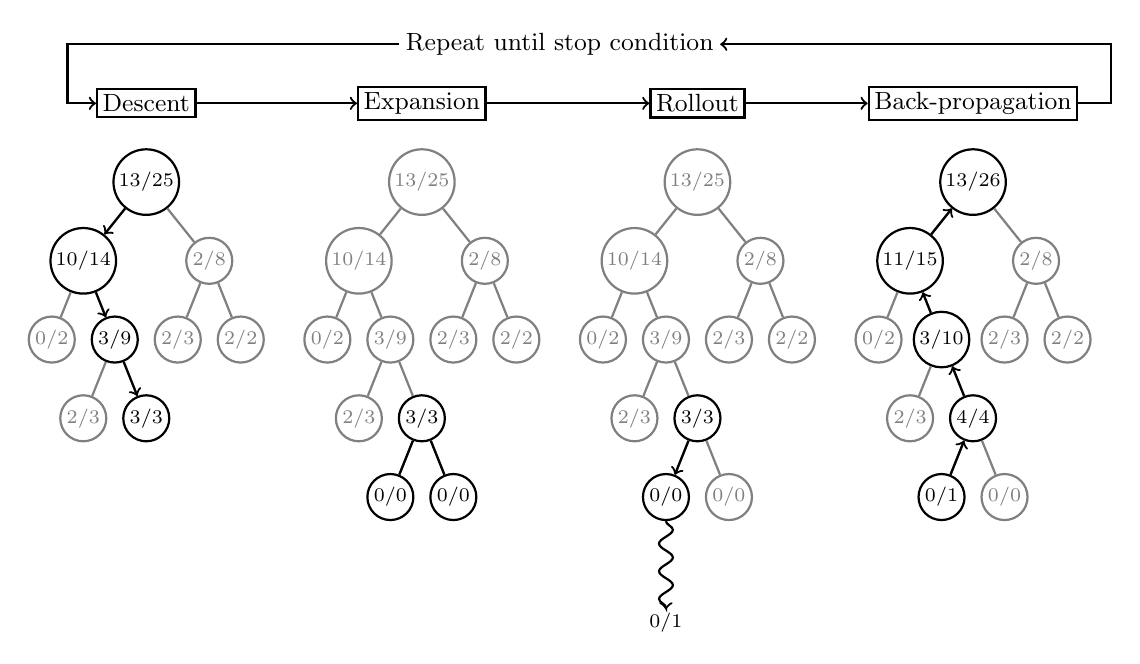
\begin{tikzpicture}
	[level distance=10mm,
	 level 1/.style={sibling distance=8mm},
	 every node/.style={gray,thick,inner sep=1pt,font=\scriptsize},
	 every path/.style={gray,thick},
	 intree/.style={draw,circle,gray,thick,inner sep=1pt,font=\scriptsize},
	 hitree/.style={draw,circle,black,thick,inner sep=1pt,font=\scriptsize},
	 desc/.style={draw,rectangle,black,thick,inner sep=2pt,font=\small},
	 scale=1 ]

\node [desc] (descent) at (0,0) {Descent};
\node [hitree] (aa) at (0,-1) {13/25}
  child {node (ab) [hitree] {10/14}
    child {node (ad) [intree] {0/2}}
    child {node (ae) [hitree] {3/9}
      child {node (ah) [intree] {2/3}}
      child {node (ai) [hitree] {3/3}}
    }
  }
  child [missing]
  child {node (ac) [intree] {2/8}
    child {node (af) [intree] {2/3}}
    child {node (ag) [intree] {2/2}}
  };
  \draw[black,->] (aa) -- (ab);
  \draw[black,->] (ab) -- (ae);
  \draw[black,->] (ae) -- (ai);


\node [desc] (expansion) at (3.5,0) {Expansion};
\node [intree] (ba) at (3.5,-1) {13/25}
  child {node (bb) [intree] {10/14}
    child {node (bd) [intree] {0/2}}
    child {node (be) [intree] {3/9}
      child {node (bh) [intree] {2/3}}
      child {node (bi) [hitree] {3/3}
        child {node (bj) [hitree] {0/0}}
        child {node (bk) [hitree] {0/0}}
      }
    }
  }
  child [missing]
  child {node (bc) [intree] {2/8}
    child {node (bf) [intree] {2/3}}
    child {node (bg) [intree] {2/2}}
  };
  \draw[black] (bi) -- (bj);
  \draw[black] (bi) -- (bk);


\node [desc] (rollout) at (7,0) {Rollout};
\node [intree] (ca) at (7,-1) {13/25}
  child {node (cb) [intree] {10/14}
    child {node (cd) [intree] {0/2}}
    child {node (ce) [intree] {3/9}
      child {node (ch) [intree] {2/3}}
      child {node (ci) [hitree] {3/3}
        child {node (cj) [hitree] {0/0}}
        child {node (ck) [intree] {0/0}}
      }
    }
  }
  child [missing]
  child {node (cc) [intree] {2/8}
    child {node (cf) [intree] {2/3}}
    child {node (cg) [intree] {2/2}}
  };
  \node (cl) [black, below of=cj,yshift=-6mm] {0/1};
  \draw[black,->] (ci) -- (cj);
  \draw[decorate,decoration=snake,->,black] (cj)--(cl);


\node [desc] (backprop) at (10.5,0) {Back-propagation};
\node [hitree] (da) at (10.5,-1) {13/26}
  child {node (db) [hitree] {11/15}
    child {node (dd) [intree] {0/2}}
    child {node (de) [hitree] {3/10}
      child {node (dh) [intree] {2/3}}
      child {node (di) [hitree] {4/4}
        child {node (dj) [hitree] {0/1}}
        child {node (dk) [intree] {0/0}}
      }
    }
  }
  child [missing]
  child {node (dc) [intree] {2/8}
    child {node (df) [intree] {2/3}}
    child {node (dg) [intree] {2/2}}
  };

  \draw[black,->] (db) -- (da);
  \draw[black,->] (de) -- (db);
  \draw[black,->] (di) -- (de);
  \draw[black,->] (dj) -- (di);


\draw[black,->] (descent) -- (expansion);
\draw[black,->] (expansion) -- (rollout);
\draw[black,->] (rollout) -- (backprop);

\node [black,inner sep=2pt,font=\small] (simulation) at (5.25,0.75) {Repeat until stop condition};
\draw[black,->] (simulation) -- (-1,0.75) -- (-1,0) -- (descent);
\draw[black,->] (backprop) -- (12.25,0) -- (12.25,0.75) -- (simulation);


\end{tikzpicture}

\end{document}

